\chapter{Results}

\section{PCA analysis of population genetics}
Based on the Principal component analysis(PCA)of 100 patients genotype information, there were no significant principal component.components.  The principal component 1 (PC1) and PC2 explained nearly the same percentage (20.17\% and 20.1\%, respectively) of genotype variation. As the methods part mentioned, the first 5 PCs were used as covariates for eQTL mapping.

\textbf{
\begin{figure}[h]
\centering
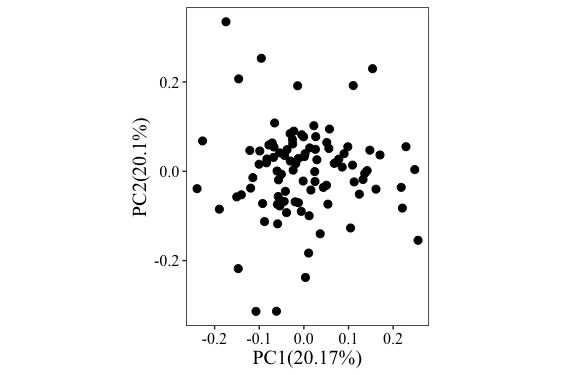
\includegraphics[width=0.8\textwidth]{figures/pca.png}
\caption{The figure illustrates the PCA plot for genotypes for 100 Japanese patients. The PC1 and PC2 are displayed on the x-axis and y-axis, respectively.}
\end{figure}
}
\section{Tumor tissue total variants}
A total of 284774 variants were called in Japanese ccRCC cohort tumor samples, including 244803 SNPs, 17346 insertions, and 22625 deletions. There were 0.182\% of variants annotated with a ‘HIGH’ impact, which means that the variant causes deleterious gene effects as determined by SnpEff. Similarly, nonsense mutations only accounted for 0.366\% of all mutations. Most of the mutations belong to missense(47.19\%) and silent mutations(52.445\%). The Transition/Transversion ratio was 2.37. As for the location of the mutations, the majority of mutations were found in introns (53.19\%). The percentage of exonic mutations is 13.24\%.The mutations also appeared in the upstream and downstream regions which occupied 12.34\% and 16.51\% , respectively.

\section{Somatic mutations in the Japanese cohort}

Only mutations remained after running FilterMutectCalls were used for statistics and downstream analysis. A total of 23997 somatic variants were remained, including 21046 SNPs,352 Multiple-nucleotide polymorphism(MNPs),610 insertions, and 1989 deletions. Variants with ‘HIGH’ impact represent 2.32\% of total somatic mutations. Missense mutations accounted for a greater proportion of the mutations (71.281\%) than silent mutations (24.753\%). The somatic mutation load in 100 patients was shown in Figure\ref{Somatic_load}. Most of the patients have around 250 to 400 somatic variants which are log-transformed to 2.4-2.6. A total of 712 mutated genes with at least five recurrent mutations have been identified. BAGE2, a long non-coding RNA (lncRNA) gene often related to melanoma, had the highest frequency of somatic mutations (67 times). The second most frequent mutated gene was VHL (54 times). The third most frequent mutated gene was TTN (51 times), which encodes protein Titin. Also, other 3 genes including PBRM1(44 times), SETD2(15 times), and BAP1(12 times) that have previously been reported in most of the ccRCC cases and studies were also identified. Except for the genes as mentioned earlier, the somatic mutated genes in this Japanese cohort, including MUC16 (33 times), MTOR (16 times), DNAH9 (12 times), HMCN1 (15 times) and KDM5C (7 times) are also ranked as top 10 mutated genes based on The Cancer Genome Atlas (TCGA) ’s ccRCC data.

The highly recurrent mutated protein-coding genes that both identified by Mutect2 algorithm and the original paper by Yusuke et. al\cite{sato_integrated_2013} includes TTN, MUC16, RYR2, CSMD3, DNAH11, LRP1B, TPTE, CSMD1, LRP2, MTOR, PKHD1, etc. A detailed somatic mutation table is available in the appendices\ref{sec:Appendices}.


\begin{figure}[h]
\centering
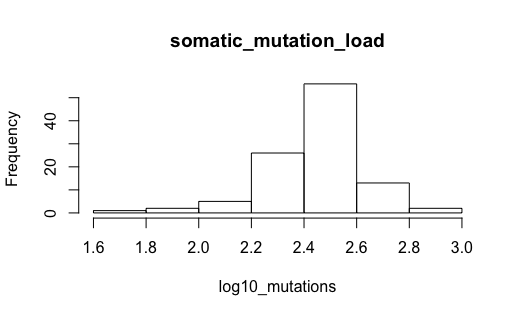
\includegraphics[width=0.8\textwidth]{figures/somatic_mutation_load.png}
\caption{The log$_{10}$ transformed somatic mutation load in 100 patients.}
\label{Somatic_load}
\end{figure}

\section{Japanese cohort eQTL analysis}
\label{eQTL}

A total of 25508 genes were tested, which excludes 180 genes that lack variant information. There were 805 significant eGenes with a FDR threshold below 0.05 after the permutation test. Most of the significant eQTLs for the 805 genes were located close to the transcription start site (TSS) of genes. See figure \ref{TSS} for a location distribution plot. The eQTLs that have the nearest distance(7bp) to TSS sites were chr19\_50344768\_G\_A for gene NAPSB and chr17\_15786625\_A\_G for gene MEIS3P1.

\begin{figure}[h]
\centering
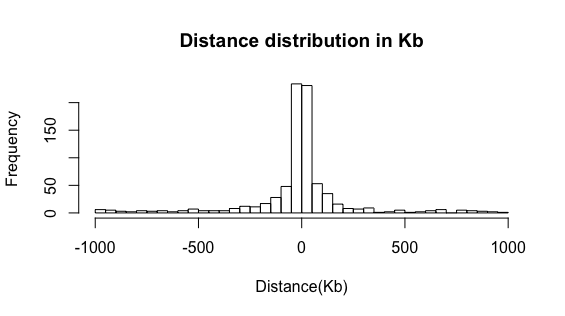
\includegraphics[width=0.8\textwidth]{figures/TSS.png}
\caption{Distance distribution between the most significant cis-eQTL site and the gene TSS site in Kb}
\label{TSS}
\end{figure}

Ranking by q-value of each identified eGenes, the most significant eGenes includes LINC01291(ENSG00000204792.2) which located on chromosome 2,ERAP2(ENSG00000164308.16) which located on chromosome 5, RPS26(ENSG00000197728.9) which located on chromosome 12 and XRRA1(ENSG00000166435.15) which located on chromosome 11. Boxplots in Figure 3.4.2 showed gene expression variation along with those eQTLs.

\begin{figure}
\label{boxplots}
	\centering
	\subfigure[Gene LINC01291 with eQTL rs3771800]{
		\begin{minipage}[b]{0.4\textwidth}
			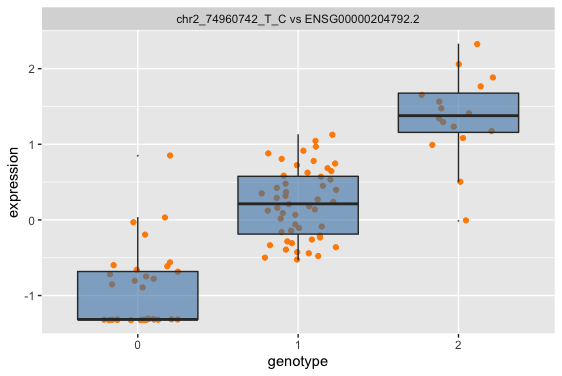
\includegraphics[width=1\textwidth]{figures/LINC01291.png} 
		\end{minipage}
		\label{fig:LINC01291}
	}
    	\subfigure[Gene ERAP2 with eQTL rs2549782]{
    		\begin{minipage}[b]{0.4\textwidth}
   		 	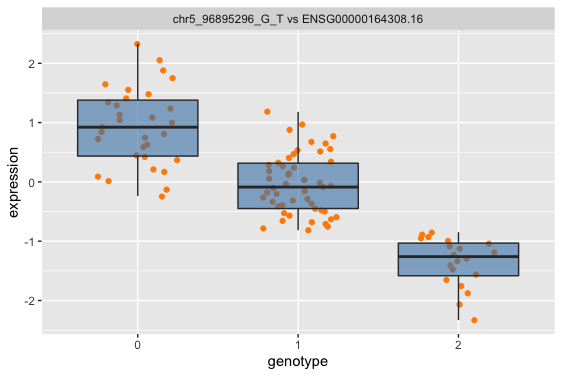
\includegraphics[width=1\textwidth]{figures/ERAP2.png}
    		\end{minipage}
		\label{fig:ERAP2}
    	}
	\\ 
	\subfigure[Gene RSP26 with eQTL rs1131017]{
		\begin{minipage}[b]{0.4\textwidth}
			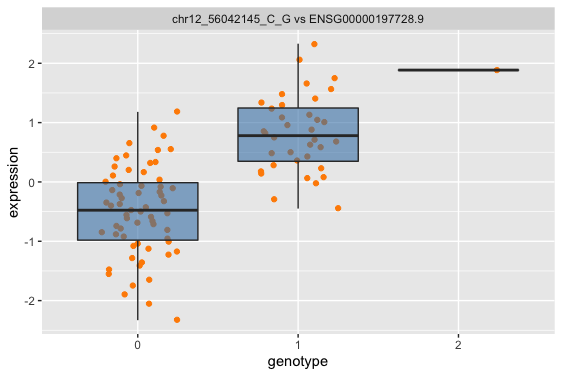
\includegraphics[width=1\textwidth]{figures/RSP26.png} 
		\end{minipage}
		\label{fig:RSP26}
	}
    	\subfigure[Gene XRRA1 with eQTL rs9787775]{
    		\begin{minipage}[b]{0.4\textwidth}
		 	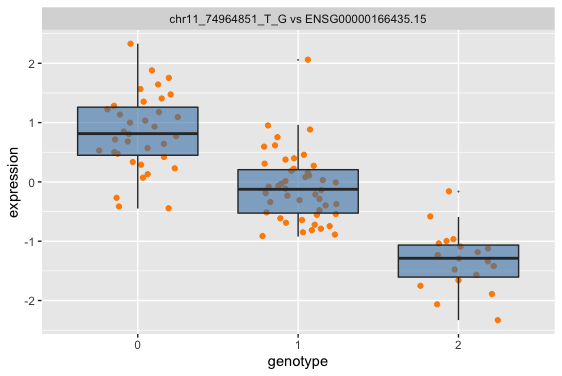
\includegraphics[width=1\textwidth]{figures/XRRA1.png}
    		\end{minipage}
		\label{fig:XRRA1}
    	}
	\caption{The representative eGenes boxplot with corresponding top eQTLs in the Japanese cohort tumor eQTL analysis}
	\label{fig:4-significant}
\end{figure}

In the GTEx published v8 release, whole genome sequencing data from 73 kidney tissues of different individuals were used and 1260 eGenes with FDR < 0.05 were identified. There were 287 eGenes that appeared in both the Japanese cohort and the GTEx V8 release, which accounts for 35.7\% of the total number of identified Japanese cancer eGenes. It is a high proportion of overlap between the eGenes that appear in GTEx databases and the eGenes identified in this study,which proved a credibility of Japanese eQTL analysis. On the other hand, 518 new significant eGenes were discovered for the Japanese cohort.

Among the 518 new eGenes, 162 of them were also identified as having somatic mutations by Mutect2 followed by FilterMutectCalls. There were also 13 significant eGenes that overlapped with highly recurrent somatic mutated genes(at least 5 times): USP24, LRRIQ3, NBPF9, FCRL3, LAMC2, ALMS1, ARFGEF3, DNAH11, PMS2P1, NUP205, RPH3A, TPP2, USP6. The detailed information was showed in table \ref{tab:13eGenes}.
\begin{table}[!ht]
\centering
\caption{13 eGenes that both significant in eQTL analysis and appeared in recurrent mutated genes}
~\\
\label{tab:13eGenes}
\resizebox{15cm}{!}{
\begin{tabular}{llllll}
\toprule
\textbf{gene name}		  & \textbf{gene chr}   &\textbf{variant id} &\textbf{rs id} &\textbf{MAF} &\textbf{qval}                            \\
\toprule
USP24 &chr1 	&chr1\_54679120\_T\_C &rs79149166 & 0.0909091 & 0.0434513\\
\midrule
LRRIQ3	&chr1 &chr1\_74205835\_A\_G	 &rs571848 &0.338384 &2.02546e-09	\\
\midrule
NBPF9 & chr1	&chr1\_149061042\_A\_C &None &0.453125 &1.05064e-12		\\
\midrule
FCRL3 	& chr1 	& chr1\_157698600\_T\_C & 	rs7522061 & 0.373737 &2.40848e-08	\\
\midrule
LAMC2 & chr1	&chr1\_183186347\_C\_A & rs684527 &0.35119 & 0.0194763\\
\midrule
ALMS1& chr2	& chr2\_74380596\_A\_G & None & 0.0104167 & 0.0134938 \\
\midrule
ARFGEF3& chr6	&chr6\_137544329\_T\_A & 	rs203693 &  0.10101 &0.021038\\ 
\midrule
DNAH11 & chr7 &chr7\_21545202\_A\_G & 	rs7781669 &  0.309278 & 1.03004e-15 \\
\midrule
PMS2P1 & chr7 &chr7\_100373690\_T\_C	 & rs2405442 & 0.479798 &5.10579e-06 \\
\midrule
NUP205	 &chr7 &chr7\_134646897\_G\_GGCT	 &None & 0.0121951 & 0.0281559 \\
\midrule
RPH3A & chr12 &chr12\_112875665\_C\_T & rs2891411 &0.444444 & 0.0253587 \\
\midrule
TPP2 & chr13 &chr13\_101692517\_A\_G & rs981073 & 0.0151515 & 0.0181033 \\
\midrule
USP6 & chr17 &chr17\_5461303\_CTTCT\_C & rs199685469 & 0.0159574 & 	0.0186372 \\
\bottomrule
\end{tabular}
}
\end{table}

See figure\ref{Overlap} for a detailed technical description and eGene counts.

\begin{figure}[h]
\centering
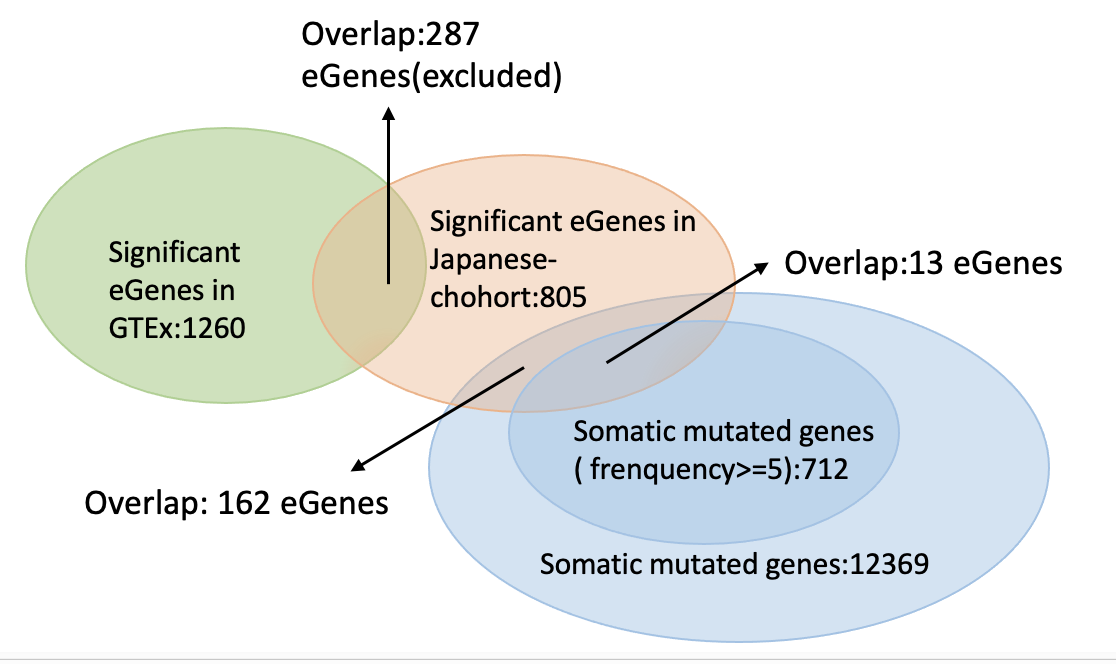
\includegraphics[width=0.8\textwidth]{figures/Overlap.png}
\caption{The study role of finding overlapped eGenes}
\label{Overlap}
\end{figure}

After the variant filtration and association tests, the top eQTLs for each significant eGene was provided in the final eQTL results table, which is available in the appendices\ref{sec:Appendices}. The lowest number of tested variants was 4 sites (for eGene MAS1L and TJP1), and the highest number of tested variants was 1040 sites (for eGene ZNF468). Besides, all the significant gene-SNP pairs were provided in another table in the appendices \ref{sec:Appendices}.



\section{Enrichr results}
The 13 eGenes and 162 eGenes described in section \ref{eQTL} were submitted to Enrichr Gene set enrichment analysis (GSEA). For the 13 highly recurrent mutated eGenes, the most significantly enriched pathway was Extracellular matrix(ECM) receptor interaction (p-value = 0.05) based on KEGG 2019 human. The gene LAMC2 was enriched in this pathway. For the 162 eGenes, the most significantly enriched pathway was Homologous recombination(HR)(p-value = 0.04).The genes BABAM1 and RAD52 were enriched in this pathway.

